\renewcommand{\theequation}{\theenumi}
\begin{enumerate}[label=\arabic*.,ref=\thesubsection.\theenumi]
\numberwithin{equation}{enumi}

\item Draw $ABCD$ with $AB=a=4.5, BC  =b=5.5, CD =c= 4, AD =d=6$ and $AC=e = 7$.
\\
\solution Fig. \ref{fig:quad_ex} shows a rough sketch of $ABCD$. Letting
\begin{align}
\label{eq:tri_basic_new}
\vec{C} = \myvec{p\\q}, \vec{A} = \myvec{0\\0}, \vec{B} = \myvec{a\\0}
\end{align}
%
it is trivial to sketch $\triangle ABC$ from  Problem \ref{prob:tri}.
%
$\triangle ACD$ is can be obtained by rotating an equivalent triangle with $AC$ on
the $x$-axis by an angle $\theta$ with
\begin{align}
\label{eq:tri_basic_rot}
\vec{D} = \myvec{h\\k}, \vec{A} = \myvec{0\\0}, \vec{C} = \myvec{e\\0}
\end{align}
%
and
\begin{align}
\label{eq:tri_rot_ang}
\cos \theta = \frac{a^2+e^2-b^2}{2ae}
\\
\sin \theta = \sqrt{1-\cos^2\theta}
\end{align}
%
The coordinates of the rotated triangle $ACD$ are
\begin{align}
\label{eq:tri_rot_trans}
\vec{D} = \vec{P}\myvec{h\\k}
\\
\vec{A} = \vec{P}\myvec{0\\0}
\\
\vec{C} = \vec{P}\myvec{e\\0}
\end{align}
%
where 
\begin{align}
\label{eq:tri_rot_mat}
\vec{P} = \myvec{\cos\theta & -\sin \theta\\ \sin \theta & \cos \theta}
\end{align}
\begin{figure}[!ht]
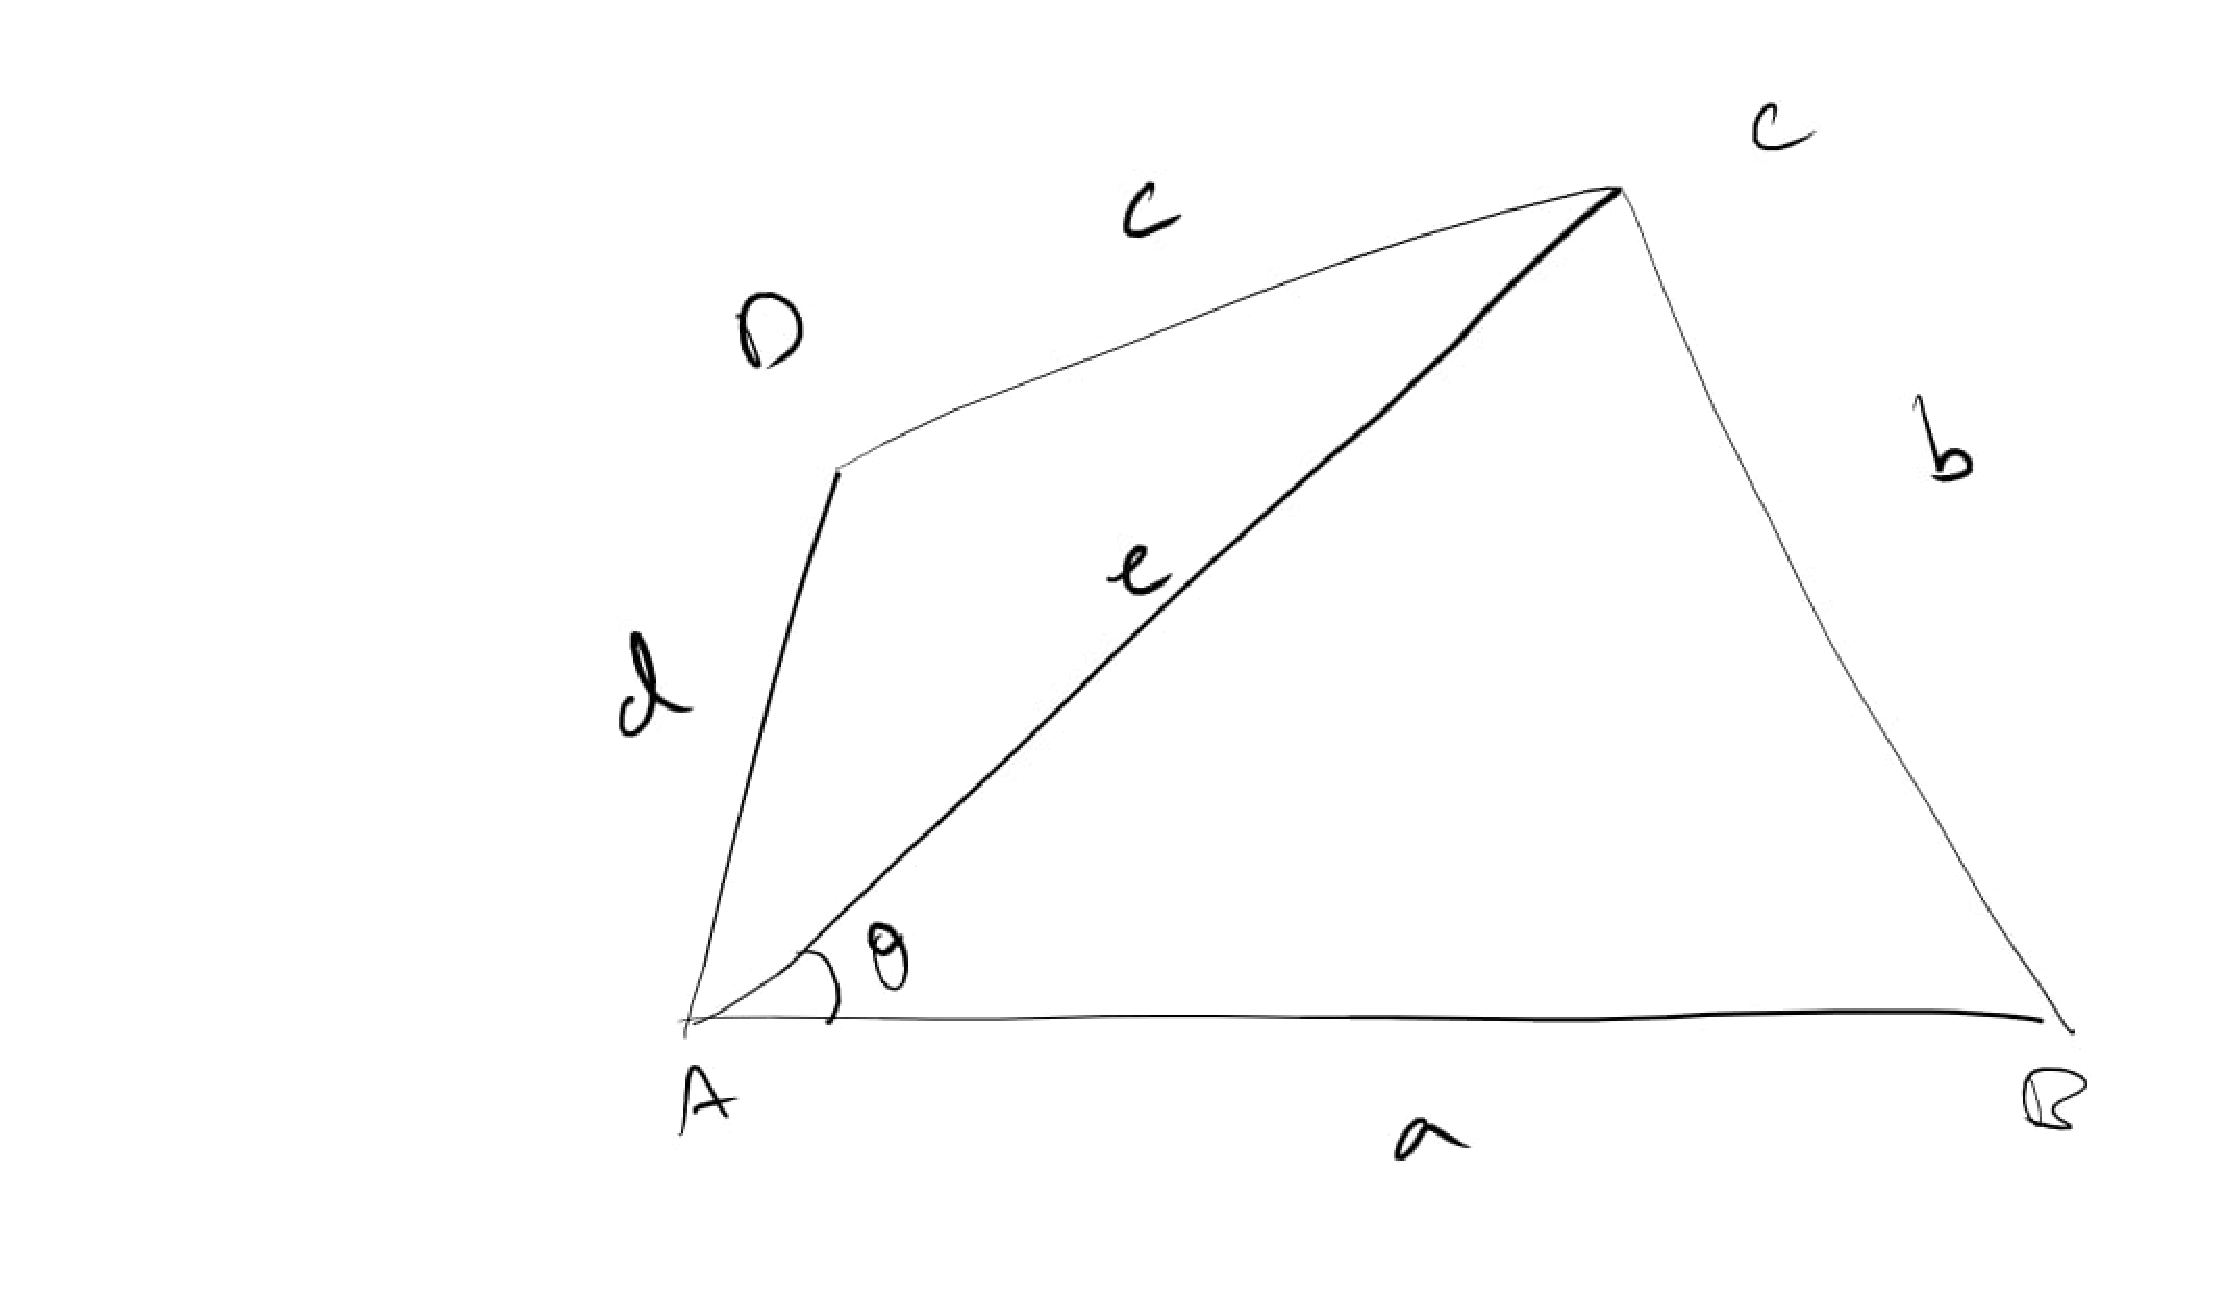
\includegraphics[width=\columnwidth]{./constructions/figs/quad_ex.eps}
\caption{}
\label{fig:quad_ex}
\end{figure}
The following code plots quadrilateral $ABCD$ in Fig. \ref{fig:quad}
\begin{lstlisting}
codes/draw_quad.py
\end{lstlisting}
\begin{figure}[!ht]
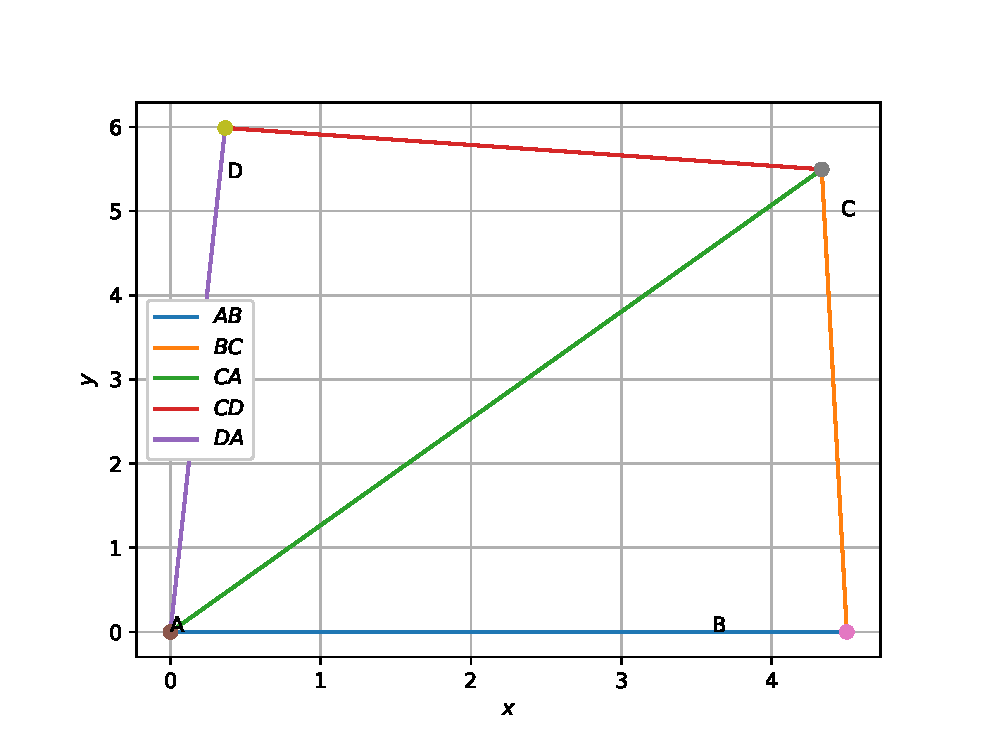
\includegraphics[width=\columnwidth]{./constructions/figs/quad.eps}
\caption{}
\label{fig:quad}
\end{figure}
\item Draw the parallelogram $MORE$ with $OR = 6, RE = 4.5$ and $EO=7.5$.
\\
\solution
Diagonals of a parallelogram bisect each other.  Opposite sides of a parallelogram are equal and parallel
.
\item Construct a kite $EASY$ if $AY = 8, EY = 4$ and $SY = 6$.
\\
\solution The diagonals of a kite are perpendicular to each other.
\item Draw the rhombus $BEST$ with $BE = 4.5$ and $ET = 6$. 
\\
\solution Diagonals of a rhombus bisect each other at right angles.


\end{enumerate}
%
